\chapter{Computational models of analogical reasoning}
\label{chapter:1}


\initial{I}n this first chapter, we provide an overview of various attempt to
formalize and theorize analogical reasoning, with a strong emphasis on
computational models. We will be led at the end of this chapter to the so
called Boolean analogical proportions and their use in machine learning, which
were the starting point of our research.

\section{Models without proportions}
\label{sec:models_without_proportions}

\subsection{Gentner's Structure Mapping Theory}

Probably the most influential model of analogical reasoning is the Structure
Mapping Theory (SMT), introduced by the American cognitive scientist Dedre
Gentne in \cite{Gen83}. The main feature of SMT is to consider that good
analogies are those that result from strong, deep, relations and dependencies
between the source and the target domains, rather than on some superficial
characteristics. In this regard, SMT departs from Hesse's theory in a
significant way. \todo{mettre ça dans Hesse si Hesse après}

The point of Gentner is that superificial similarities are often irrelevent,
while what matters in an analogy are the underlying \textbf{structural}, high
order relations between the objects at play. To examplify, Gentner argues that
when one says that \textit{a battery is like a reservoir}, the analogy stands
because at some abstract level, a battery and a reservoir serve the same
purpose: to release some potential energy that has been stored for some time.
The fact that batteries come in different shapes, colors and sizes than
reservoirs does not play any role in the relevence of the analogy. This
principle is called the \textbf{systematicity principle}, for which we now give
some technical details.

The world is assumed to be represented by objects (belonging either to the
source domain $S$ or the target domain $T$), along with some
\textbf{predicates} that deal with one or more objects of the same domain. The
distinction is made between predicates that only take one argument
(\textbf{attributes} of objects), and those  that take at least two objects
(\textbf{relations}). Higher-order relations are relations for which arguments
are themselves relations, instead of simple objects. To illustrate these
syntactic distinctions, \textit{TALL(Bob)} and \textit{BLONDE(Alice)} are
attributes over the objects \textit{Bob} and \textit{Alice}.
\textit{ARE\_FRIENDS(Bob, Alice)} and \textit{HAVE\_DINNER(Bob, Alice)} are
first-order relations, and \textit{CAUSE[ARE\_FRIENDS(Bob, Alice),
HAVE\_DINNER(Bob, Alice)]} is a second-order relation.

In SMT, an analogy is defined as a one-to-one mapping $M$ from $S$ to $T$ that maps
relations (and only relations) between the two domains. The systematicity
principle mentioned earlier states that during the mapping, attributes of
objects (considered to be superficial features) are discarded and not taken
into account, while higher-order relations are given priority over lower-order
ones. Also, out of two relations of the same order, the one that is the most
involved into other (higher-order) relations is the most likely to be mapped in
the target domain. This last requirement gives an implicit rule to somehow
assess the relevence of a relation in an analogy.

Note that this definition of analogy involves purely structural and syntactical
features. The semantic underlying the relations (or the objects) are competely
out of concern. In our example, the fact that \textit{Alice} and \textit{Bob}
are actually friends is of no importance: for SMT this relation is nothing but
a first-order relation, with no particular meaning. As far as SMT is concerned,
\textit{Alice} and \textit{Bob} could just as well be arch-enemies, it would
not make any difference during a potential mapping process with a target domain
(which would, for example, involve two other individuals with a similar
relationship).

While SMT is a purely theoretical framework for analogy, these ideas have been
practically implemented in a software called the Structure Mapping Engine (SME)
\cite{FalForKenGen89} written in LISP, leading to numerous
applications.\todo{Lovett?} The SME algorithm, in complete accordance with SMT,
can be conceptually summarized as follows:

\begin{enumerate}
    \item Look for all potential matches between relations in the source domain
      and the target domain.
    \item Try to group matches into maximally consistent collections of
      matches.
    \item From each collections, infer some relations that might stand in the
      target domain.
\end{enumerate}

In  \cite{ChaFreHof92}, authors point out various concerns about SMT and SME.
Among them is the fact SME is too reliant on the (human-made) description
inputs of the source and target domains, and that the intelligence mostly comes
from these descriptions:

\begin{quote}
  when the program’s discovery of the correspondences between the two situations
  is a direct result of its being explicitly given the appropriate structures
  to work with, its victory in finding the analogy becomes somewhat hollow.
  Since the representations are tailored (perhaps unconsciously) to the problem
  at hand, it is hardly surprising that the correct structural correspondences
  are not difficult to find.
\end{quote}

Also, while the systematicity principle is undoubtly at the core of many
analogies, it should seem natural to challenge it in some other situations. It
is indeed quite easy to find analogies were superficial features are the most
decisive ones \cite{Bar10}.

\subsection{Analogy and the Minimum Description Length Principle}

Ockham's razor (also Occam), due to the Franciscan philosopher William
of Ockham (1285~-~1347), is a well known principle in machine learning theory.
The main and most useful interpretation of the original latin version states
that when trying to explain a situation, if two hypothesis give the same answer
then the best one is probably the \textbf{simplest} one. In practice, what
makes an hypothesis simple remains quite vague, at least from a computational
point of view. Yet this principle has been formalized into Rissanen's Minimum
Description Length Principle (MDLP) \cite{Ris78}, which is based on Kolmogorov
complexity. Despite the difficulty to build inferential models from this
principle (Kolmogorov complexity is often intractable and impossible to
compute or even to estimate), it has shown to be quite influential in the field
of machine learning, at least from a theoretical point of view.

With this in mind, Antoine Cornuéjols proposed a framework for assessing the
quality of an analogy \cite{CorMLS96} (see also \cite{CorJFA96}).\todo{Faire lien
entre ça et AD de Miclet} In these papers, Cornuéjols hypothesizes that the
best analogy between a source and a target model is the one that minimizes its
description length, in terms of Kolmogorov complexity.

Let us first first recall some basic knowledge about Kolmogorov complexity,
before diving into more technical details. The Kolmogorov complexity of a
string of characters $x$, denoted $K(x)$, is the length of the shortest
computer program capable of outputing $x$. $K(x)$ is supposed to capture the
intrinsic complexity of $x$. Intuitively, $K('aaaaabbbbb')$ is supposed to be
lower than $K('abaabbabab')$, because a clear pattern emmerges in the first
string, leading to a simple program: first print $a$ five times, then do the
same for $b$. The second string seems more or less random, which makes it
difficult to factorize into a concize program. In somse sense, the Kolmogorov
complexity captures how well can a string $x$ be \textit{compressed}. The
conditional complexity $K(x \given y)$ is the size of the shortest program that
outputs $x$ when given $y$ as an input.

Now, let's get back to our analogical concerns. As illustrated in figure
\ref{FIG:cornuejols_model}, Cornuéjols considers an analogy as a process
involving an object $x_S$ in a source domain, an object $x_T$ in a target
domain, and two functions $f_S$ and $f_T$ transforming $x_S$ and $x_T$ into
$y_S$ and $y_T$ respectively: $y_S = f_S(x_S)$ and $y_T = f_T(x_T)$. Each
domain $S$ and $T$ \textit{lives} inside a theory or model (namely $M_S$ and
$M_T$), that can describe their corresponding objects.

\begin{figure}[!h]
\centering
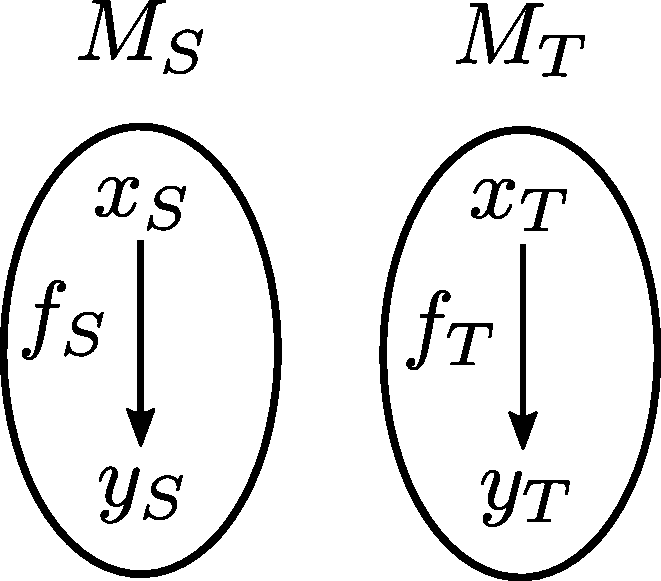
\includegraphics[width=1.5in]{figures/cornuejols_model.pdf}
\caption{The two domains $S$ and $T$ in Cornuejols' model.}
\label{FIG:cornuejols_model}
\end{figure}

For Cornuéjols, the best analogy is the one that minimizes the following sum of
Kolmogorov complexities:
$$K(M_S) + K(x_S \given M_S) + K(f_S \given M_S) + K(M_T \given M_S) + K(x_T
\given M_T) + K(f_T \given M_T),$$
where:
\begin{itemize}
   \item $K(M_S)$ is the cost associated with the source theory,
   \item $K(x_S \given M_S)$ is the cost of $x_S$ as described in the source
     theory,
   \item $K(f_S \given M_S)$ is the cost of $f_S$ as described in the source
     theory,
   \item $K(M_T \given M_S)$ is the cost of describing the target theory from
     the source theory,
   \item $K(x_T \given M_T)$ is the cost of $x_T$ as described in the target
     theory,
   \item and finally $K(f_T \given M_T)$ is the cost of $f_T$ as described in
     the target theory.
\end{itemize}

Notice that the terms $y_i$ are not considered in this cost function, because
they are entirely defined by their corresponding $x_i$ and $f_i$.

parler des applications mais sans doute après COPYCAT?
